\subsection{Software Platforms}
The LEGO NXT is a flexible platform, as it allows for custom firmware to be installed, which in turn allows for different programming languages to be used.
Some of these include RobotC\cite{RobotC}, leJOS\cite{leJOS} and nxtOSEK\cite{nxtOSEK}.

\subsubsection{NXT-G}
NXT-G is the development environment supplied with the LEGO NXT. NXT-G is a programming language based on LabView\cite{LabView}. The language uses drag and drop block programming, instead of writing code, illustrated in figure \ref{NXT-G}. This gives NXT-G a fast learning curve and development environment. Furthermore it provides a visual representation of the program, but just as the representation is very abstract so is the programming opportunities. This means NXT-G is very limited when it comes to low level programming, and more complex programs.


% Despite the NXT ship with the NXT-G programming language. NXT-G is a programming language based on LabView\cite{LabView}. The language uses a drag and drop block system, instead of writing code, illustrated in figure \ref{NXT-G}. This also provides a visual representation of the program.

\begin{figure}[H]
    \centering
    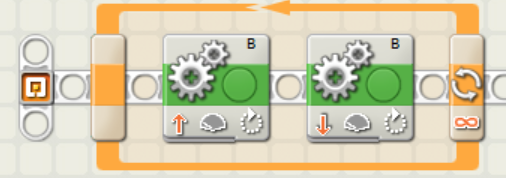
\includegraphics[width=0.7\textwidth]{Images/Software/Mindstorms/mindstorms_block.png}
    \caption{Illustration of two motor blocks running in a loop in NXT-G.}
    \label{NXT-G}
\end{figure}

% This approach is easier to understand, but is limited when it comes to low level programming and when creating more complex programs. Luckily the NXT is a flexible platform, as it allows for custom firmware to be installed, which in turn allows for different programming languages to be used.
% Some of these include RobotC\cite{RobotC}, leJOS\cite{leJOS} and nxtOSEK\cite{nxtOSEK}.

\subsubsection{RobotC}
This programming language is designed specifically for robot platforms. It is built on top of C, and with the primary purpose of being an educational platform. Noteworthy is that it is not free to use and requires a license.

\subsubsection{leJOS}
leJOS is an open-source firmware that includes the Java Virtual Machine\cite{Java}, and as such allows for writing Java programs. leJOS was originally written for the LEGO RCX, an earlier version of the NXT, it has since been updated to run on the NXT.

leJOS has plugins for both Netbeans\cite{Netbeans} and Eclipse\cite{Eclipse} for making development more convenient.

\subsubsection{nxtOSEK} \label{nxtOSEK}
nxtOSEK is a hybrid firmware of leJOS and TOPPERS\cite{TOPPERS}. nxtOSEK supports programming in C and C++, which gives nxtOSEK the possibility of very optimised code. Furthermore since nxtOSEK is based on OSEK software architecture \unsure{Brugt til biler?, ved ikke helt om det skal nævnes}.

There are three ways to run nxtOSEK on a NXT. These approaches have different pros and cons, in table \ref{firmCom} a comparison of these, can be seen.
\begin{table}[H]
    \centering
    \label{firmware-comparison}
    \begin{tabular}{|l|l|l|l|}
    \hline
    & Memory & Programs & Interface \\ \hline
    Stock Firmware & 64KB & Multiple & Stock \\ \hline
    \begin{tabular}[c]{@{}l@{}}
    John Hansen's\\ Enhanced NXT Firmware\end{tabular} & 64KB & Multiple & Stock \\ \hline
    NXTBios & 
    \begin{tabular}[c]{@{}l@{}}224KB ROM\\ 50KB RAM\end{tabular} & Single & Barebone \\ \hline
    \end{tabular}
    \caption{Comparison between firmware}
    \label{firmCom}
\end{table}

nxtOSEK supports scheduling using priority based scheduling\todo{reference needed}. It uses alarms to define priorities and the execution rate.

\subsection{Choice of software}


We have chosen to use the nxtOSEK because it does not cost us any money, it has the functionality that we need, and it allows for sufficiently low level programming languages, which is important when real-time systems are considered.


% Ikke analyseret så mange
% nxtOsek fordi det er gratis               RobotC
% support for scheduling
% Bygget på Osek som er lavede til biler.   
% supporter c++, bedre end java             leJOS
